\documentclass[final,3p,times]{article}

\usepackage{amssymb} %math symbols
%\usepackage{graphicx} %[trim]
\usepackage{graphicx,wrapfig,lipsum}
\usepackage{media9}
\usepackage{enumerate}
%make paragraph look like section
\usepackage{titlesec}
\titleformat{\paragraph}[hang]{\normalfont\normalsize\bfseries}{\theparagraph}{1em}{}
\titlespacing*{\paragraph}{0pt}{3.25ex plus 1ex minus .2ex}{1em}
\usepackage{enumitem}
\usepackage[a4paper, total={6in, 8in}]{geometry}
\usepackage{titling}
\usepackage{subfig}

\begin{document}

\title{Robotics101}
\author{Sergio Azizi}
\date{September 23, 2016}
\maketitle

\paragraph{Foreword}
The objective of this project was to build a low-cost robot, which can (a) detect and avoid obstacles, and (b) 
follow a source of light. \\
I completed this project with the UCLU Robotics Society.\\
This document is just a brief, informal summary of the project \\
\begin{tiny}
(and my first ever attempt at using latex...have mercy on me and the amateur formatting).
\end{tiny}

\paragraph{Mission}
Build a robot that that will follow a light source while avoiding obstacles...\\
\includemedia[width=0.4\linewidth, height=0.3\linewidth, activate=pageopen, addresource=./media/lightFollow.mp4, flashvars={source=./media/lightFollow.mp4, &autoPlay=true}]{}{VPlayer.swf}\\
...complete

\paragraph{Journey}
There are three parts to this:
\begin{enumerate}
\item Assembly
\item Obstacle Avoidance
\item Light Follower
\end{enumerate}
Overall, pretty simple.

\newpage

\section{Assembly}

\subsection{The Microcontroller}
I used an \textbf{Arduino Uno}. Here is a quick overview:
\begin{figure}[h]

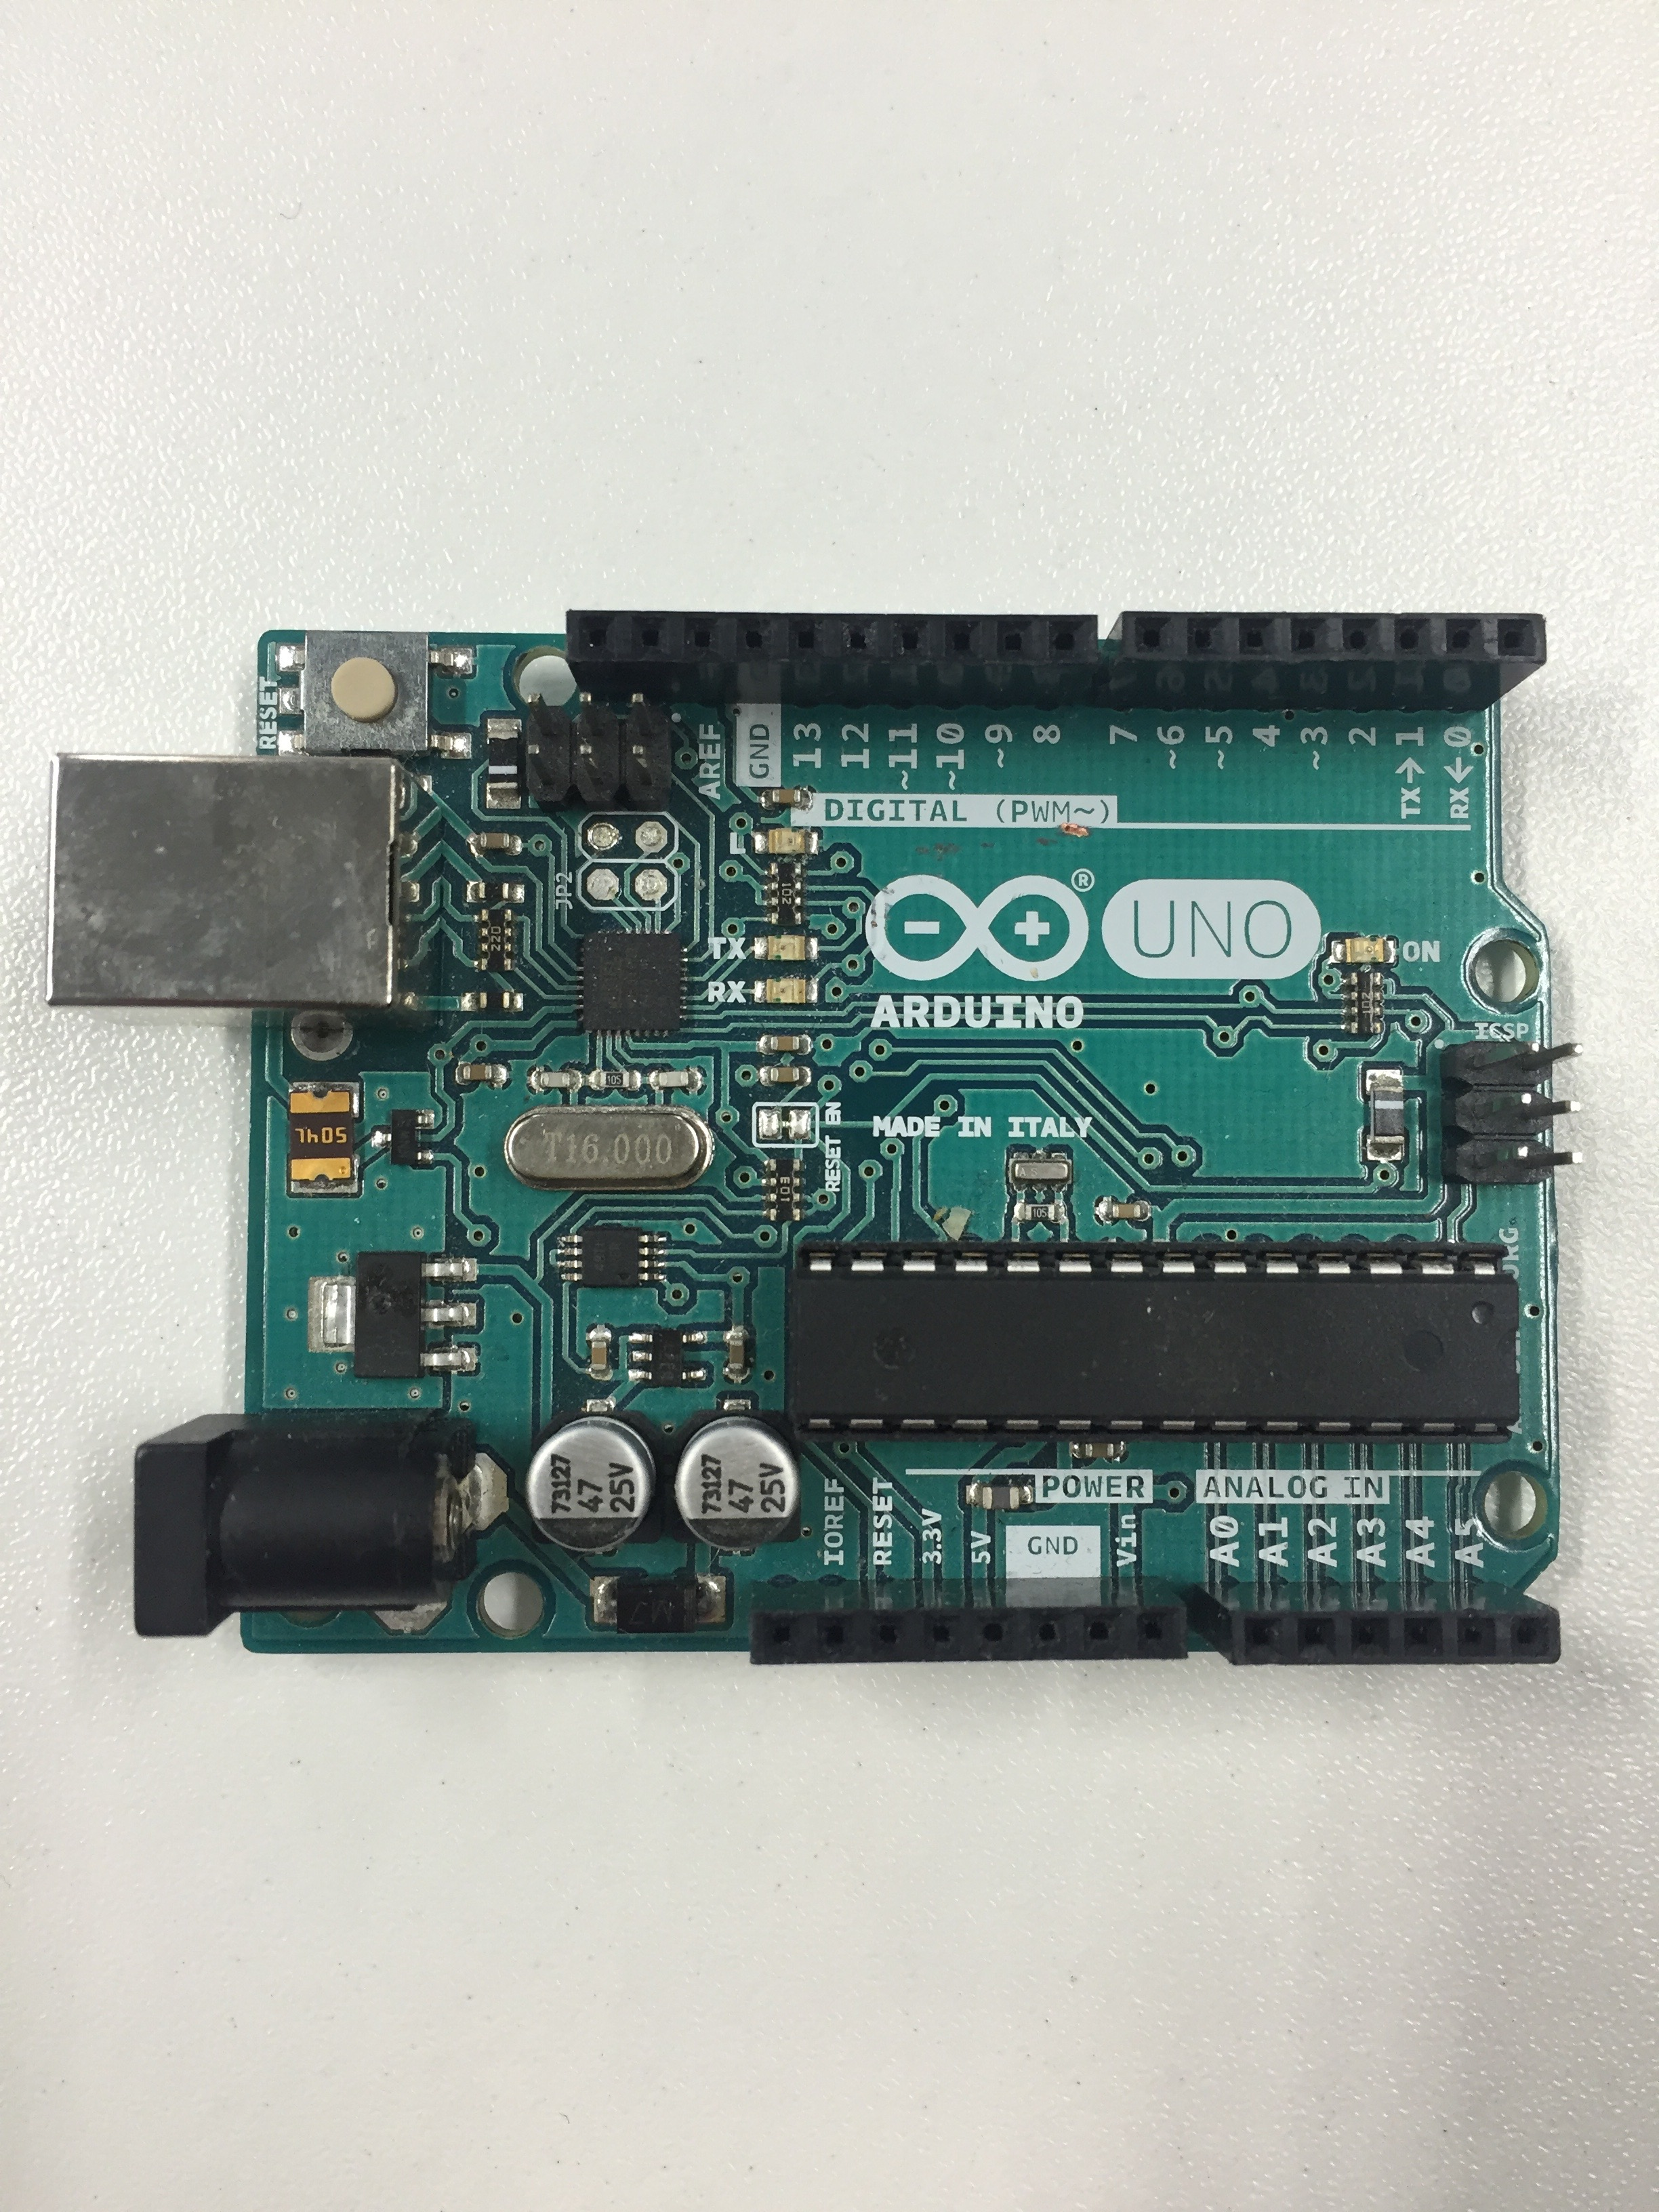
\includegraphics[trim={0 28cm 0 30cm}, clip, width=3in]{./media/microController.jpg}
\label{fig:MicroController}
\end{figure}
\begin{description}[style=unboxed,leftmargin=0cm]
\item[Pin's]
The top row are the digital pins (used with digitalRead(), digitalWrite and analogWrite).\\
In the bottom right, we have the analog pins (used with analogWrite).\\
Next to it, (bottom central), we have GND and 5V pins, to connect arduino to ground and provide +5V power.
\item[LED's]
LED 13, driven by pin 13.\\
Underneath are TX and RX LED's, indicating communication computer and Arduino.\\
To the right of the label, is the power pin (indicats if arduino receives power).\\ \\
The actual microprocessor (an ATmega) is positioned underneath the label.\\
In the bottom left is the power connector where the batteries will be attached to.
\end{description}

\subsection{controls}
The body of my "robot" is a wooden board with three wheels attached to it, two at the front and one in the back.
The front wheels are powered via two brushless DC motors.
\begin{wrapfigure}{l}{5.5cm}
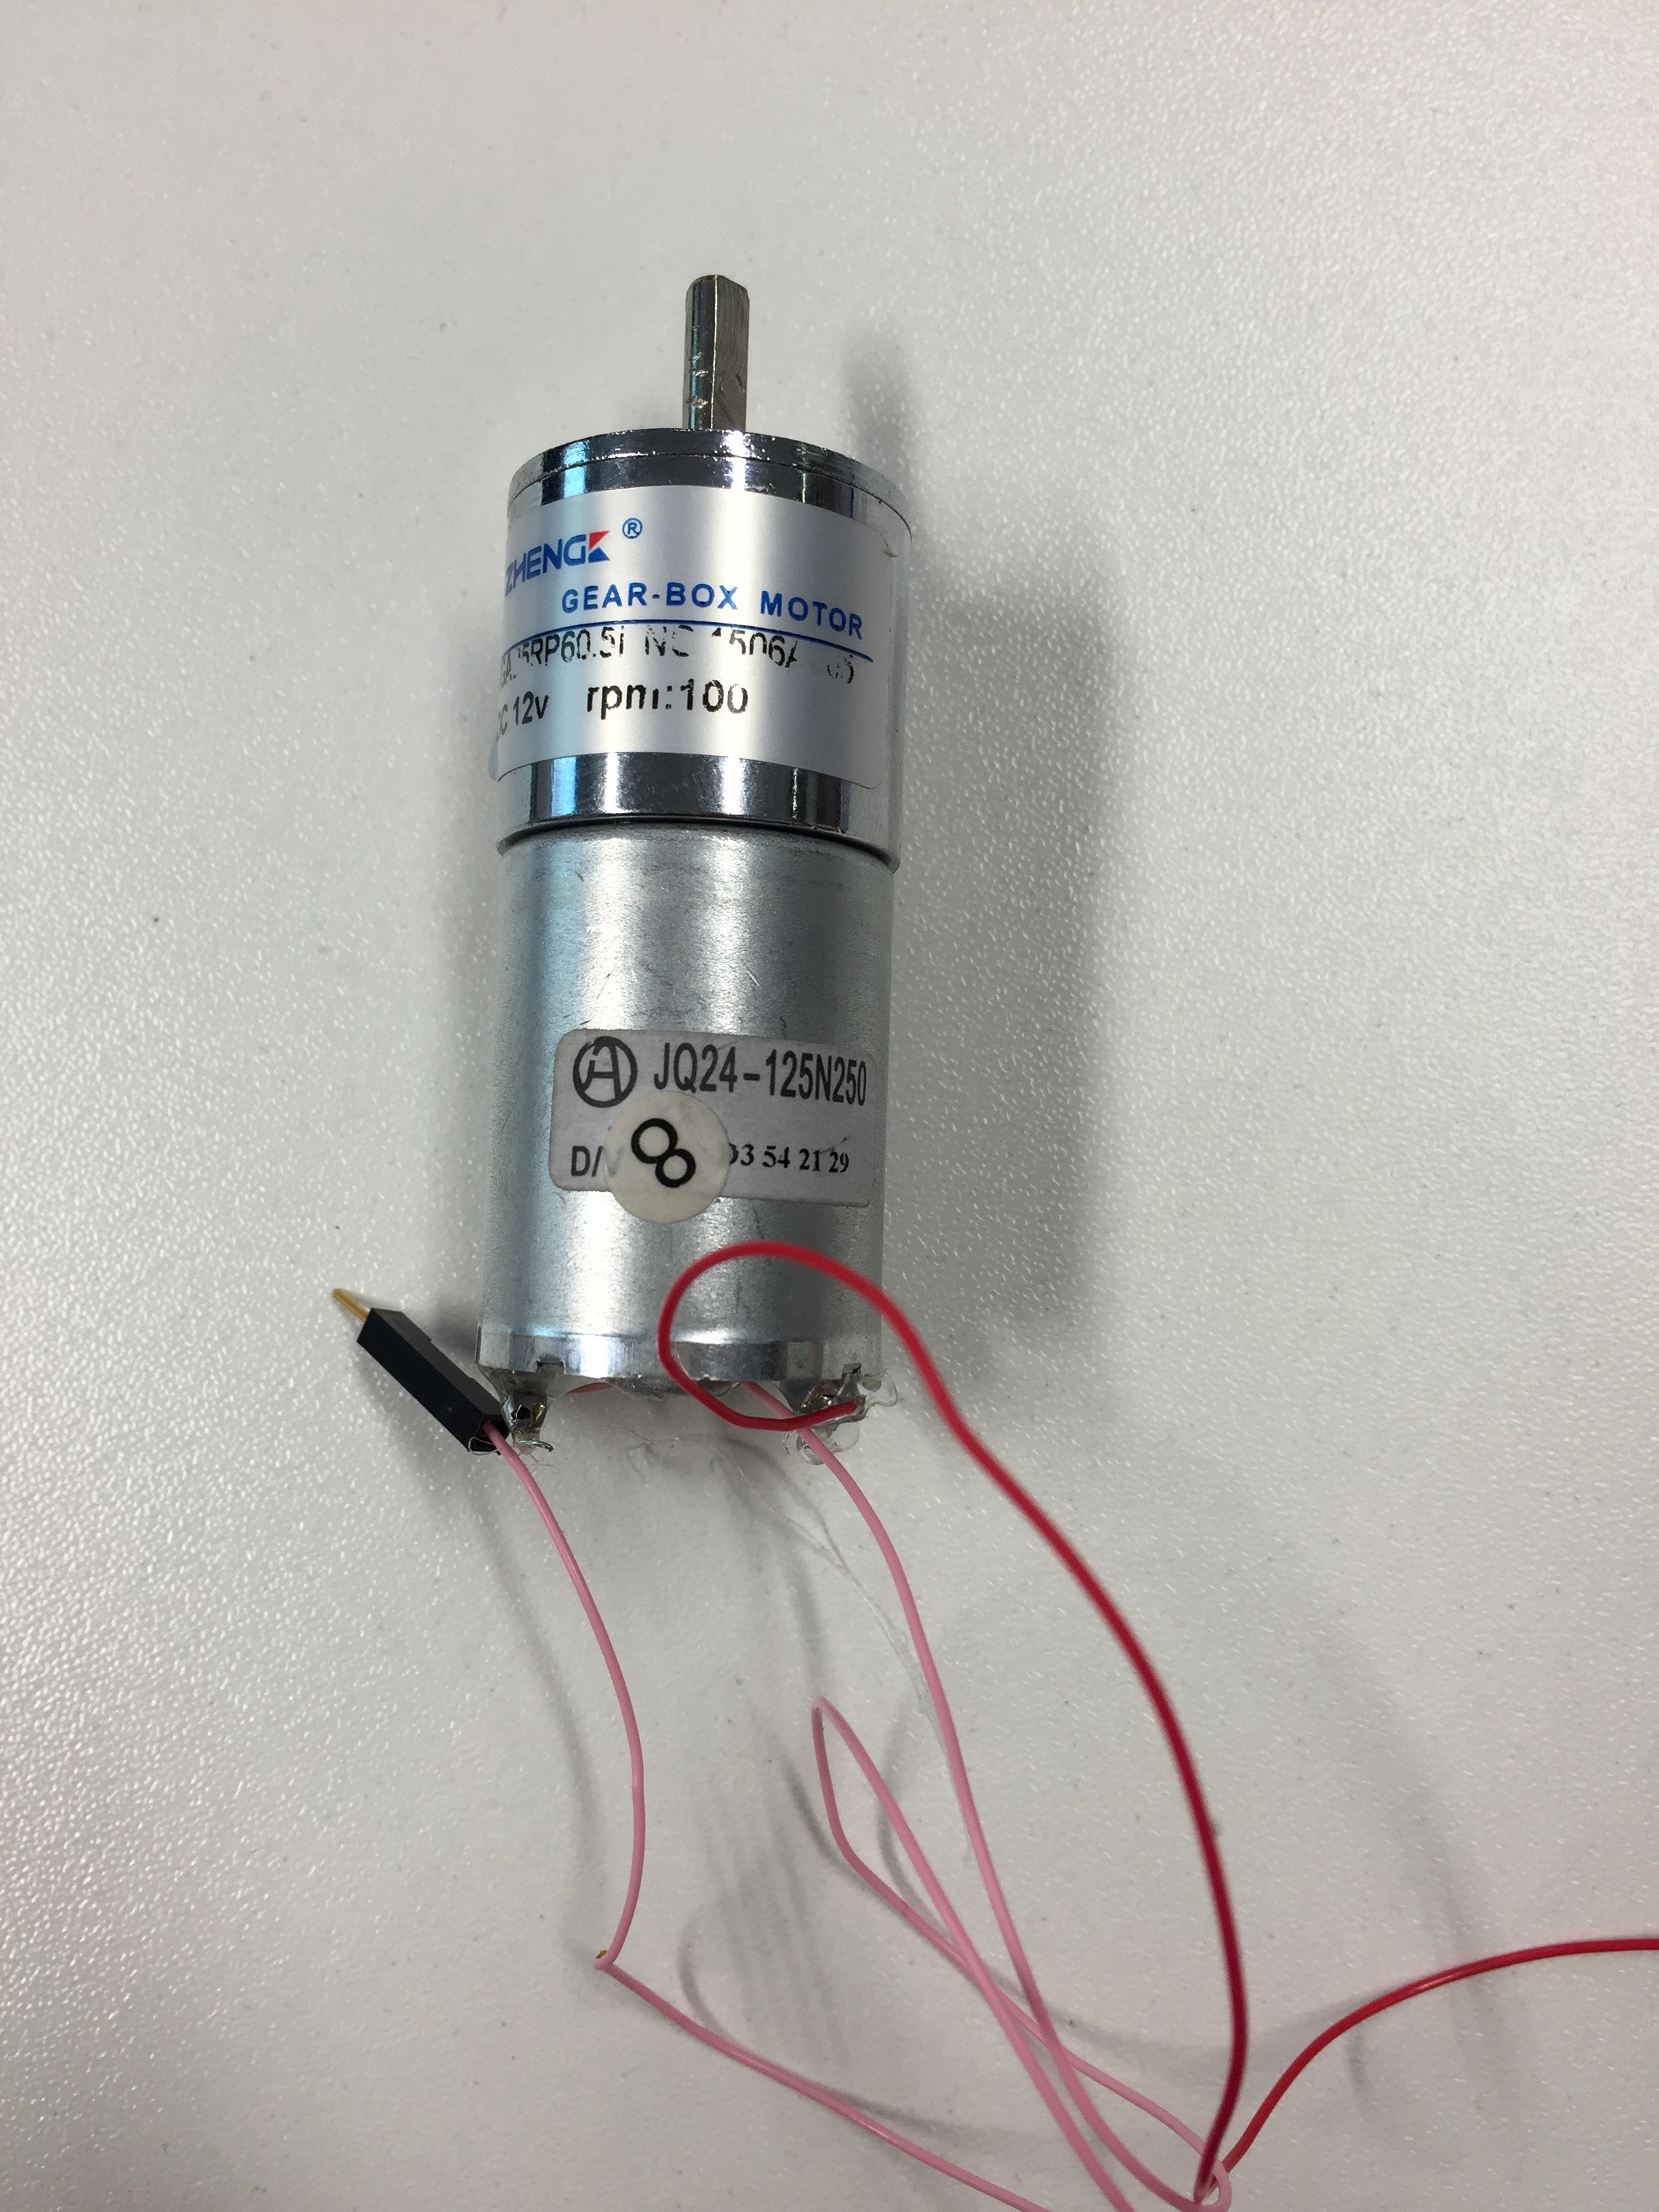
\includegraphics[trim={5cm 30cm 25cm 10cm}, clip, width=2in, height=2in]{./media/motor.jpg}
\end{wrapfigure}
Each motor requires a current of 0.5 amps and a voltage of at least 6V.
However, the \textbf{Arduino Uno} is only capable to providing 0.4 amps and 5 volts.\\
\textit{Solution}:
With a motor driver board and a switch that operates at the Arduino current and voltage level,  I control the necessary amps and volts to change directions of the rotation.\\
Operating at Arduino level means when you supply 5V it is "turned on", and when you supply 0V, it's "turned off".
Here is the concept: The Driver is is arranged like an H-Bridge:
When the switch is turned on, the circuit will close at high-left and low-right, causing the motor to rotate clockwise. Similarly, when the switch is turned off, the motor will turn in the anti-clockwise direction.
\begin{figure}[!tbp]
  \centering
  \subfloat[Driver Board.]{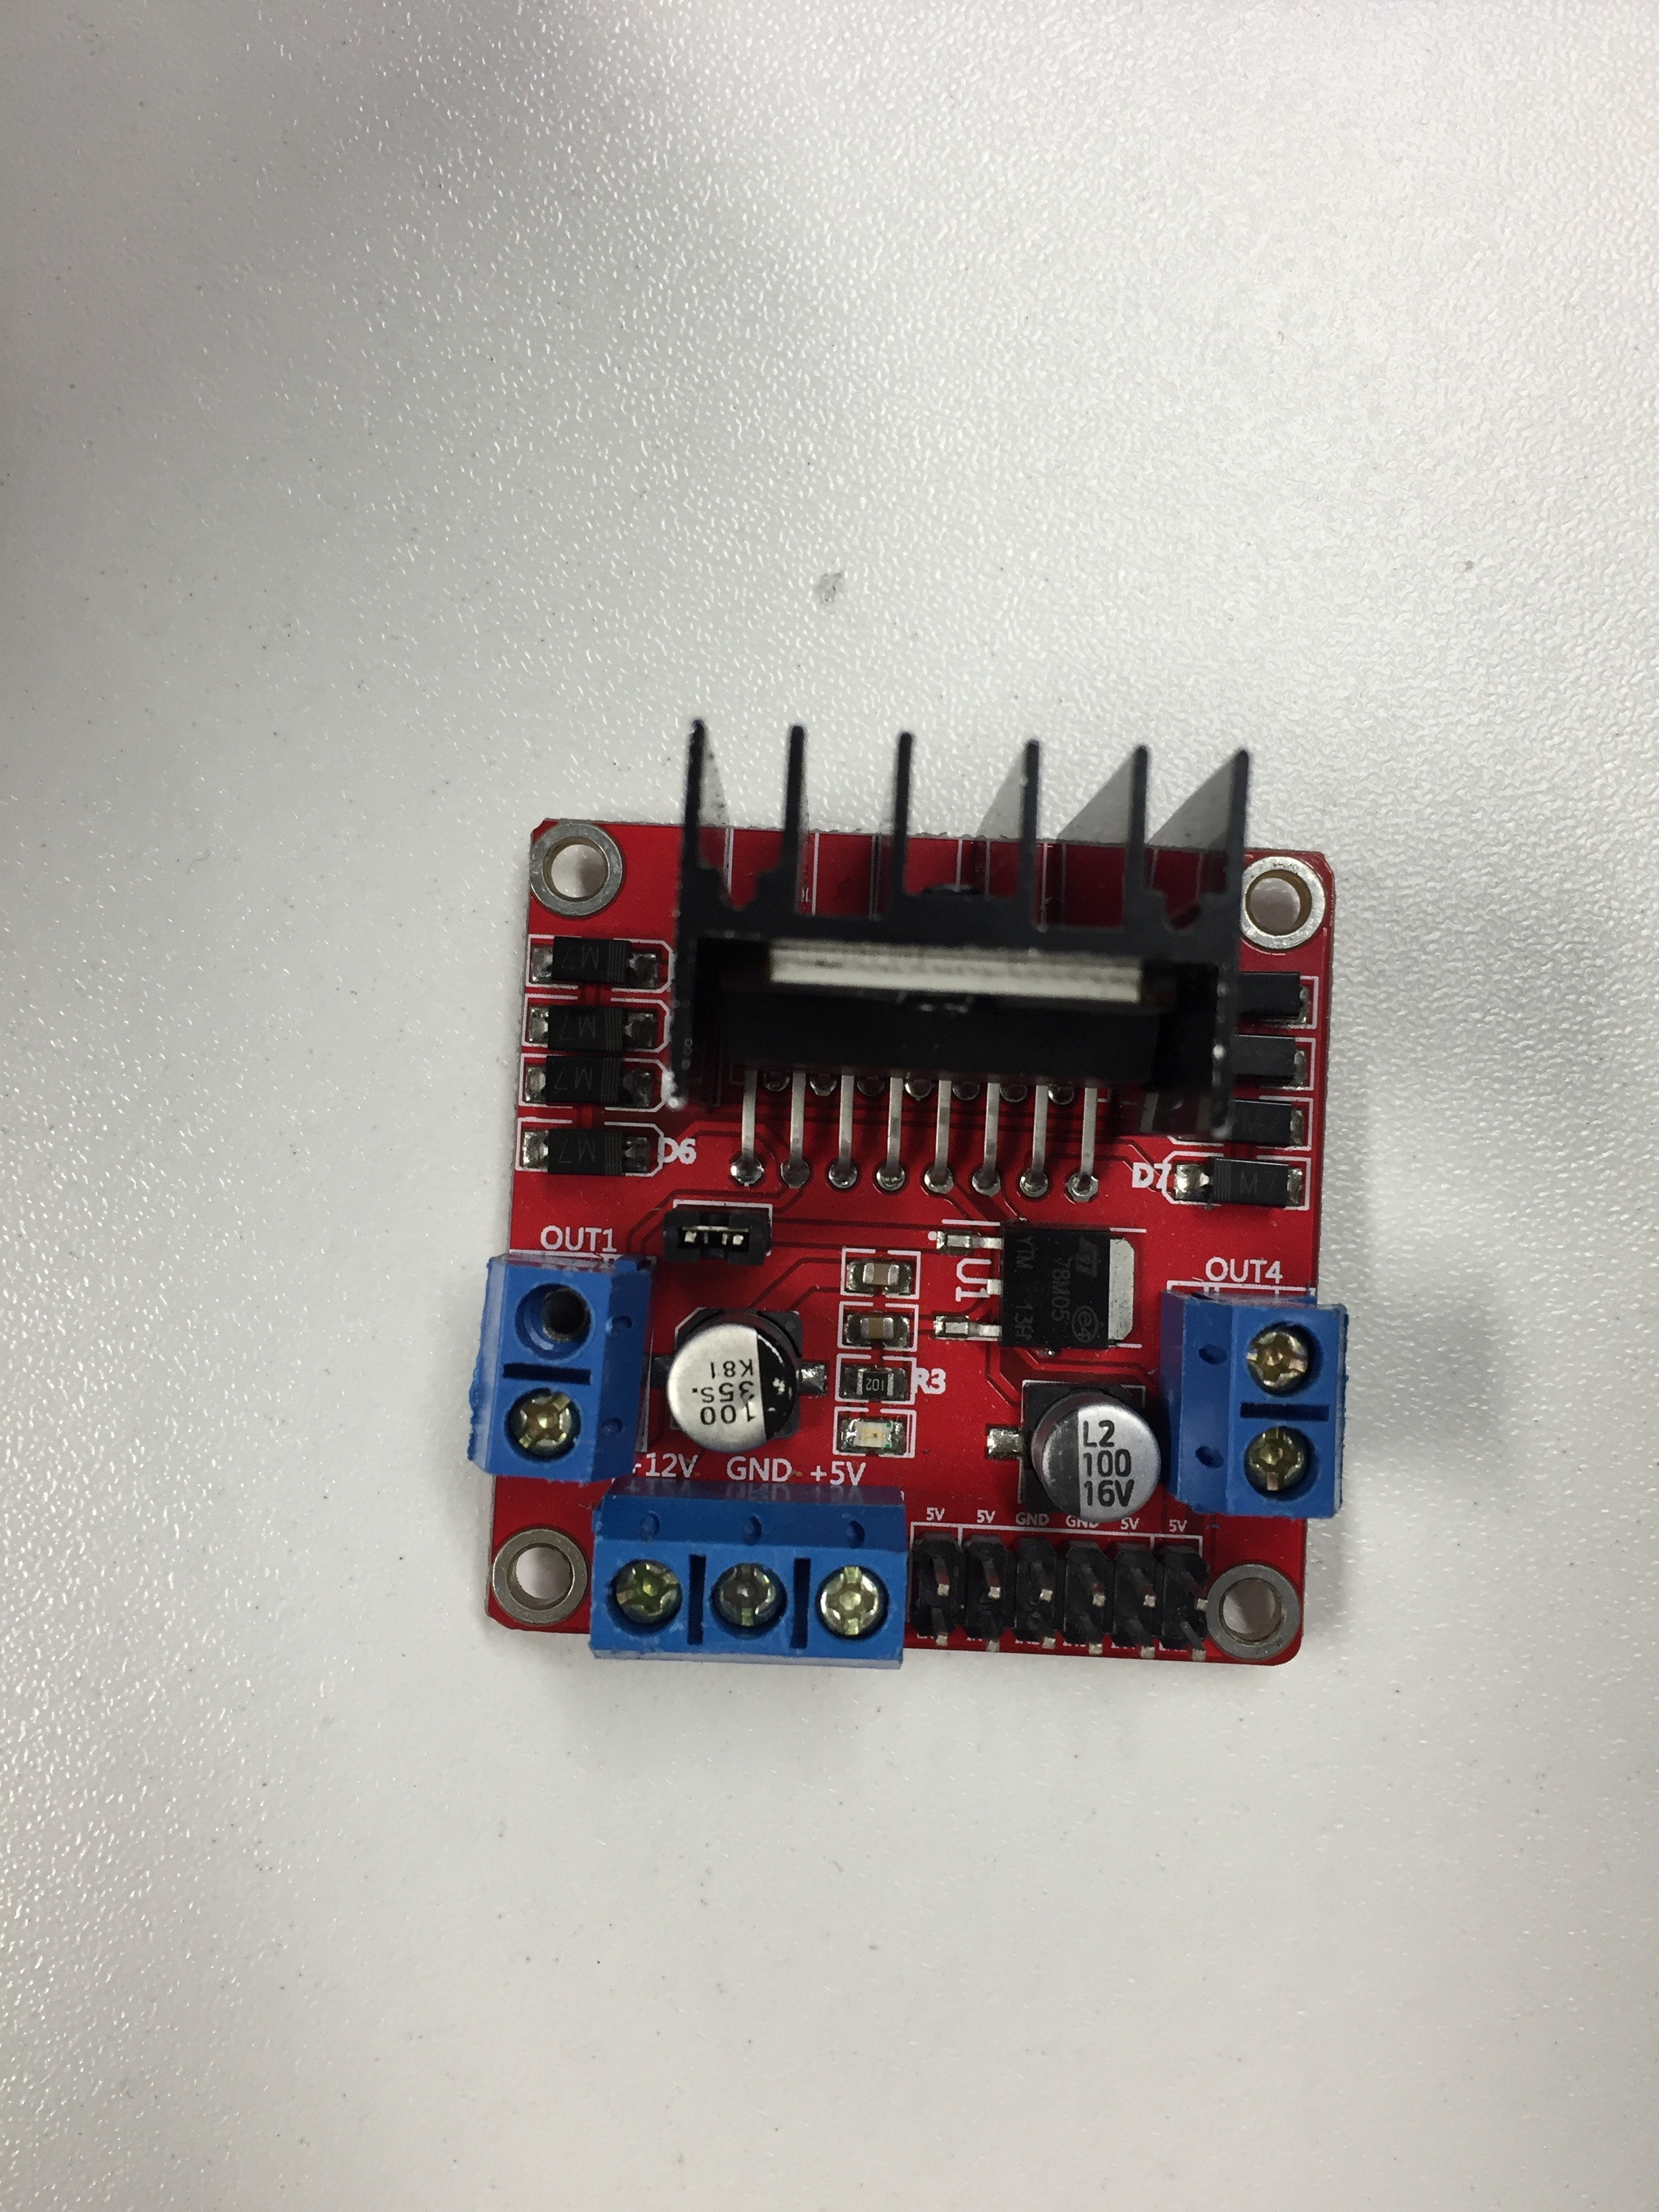
\includegraphics[trim={20cm 25cm 15cm 35cm}, clip, width=2.2in, height=2.2in]{./media/motorDriver.jpg}}
  \hfill
  \subfloat[h-Bridge.]{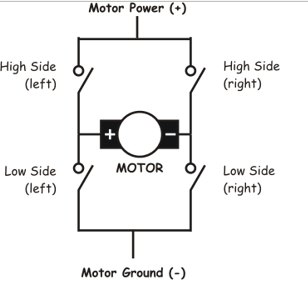
\includegraphics[trim={0cm 0.5cm 0cm 0.1cm}, clip, width=2.2in, height=2.2in]{./media/hBridge.jpg}}
\end{figure}
\\
We can then define a function like the one below and simply call left() whenever we want to do so.
\begin{figure}[!h]
\includegraphics[trim={0cm 0cm 0cm 0cm}, clip, width=3in]{./media/motorControls.jpg}
\includegraphics[trim={0cm 0cm 0cm 0cm}, clip, width=3in]{./media/goLeft.jpg}
\end{figure}

\section{Obstacle Avoidance}
\begin{figure}[h]
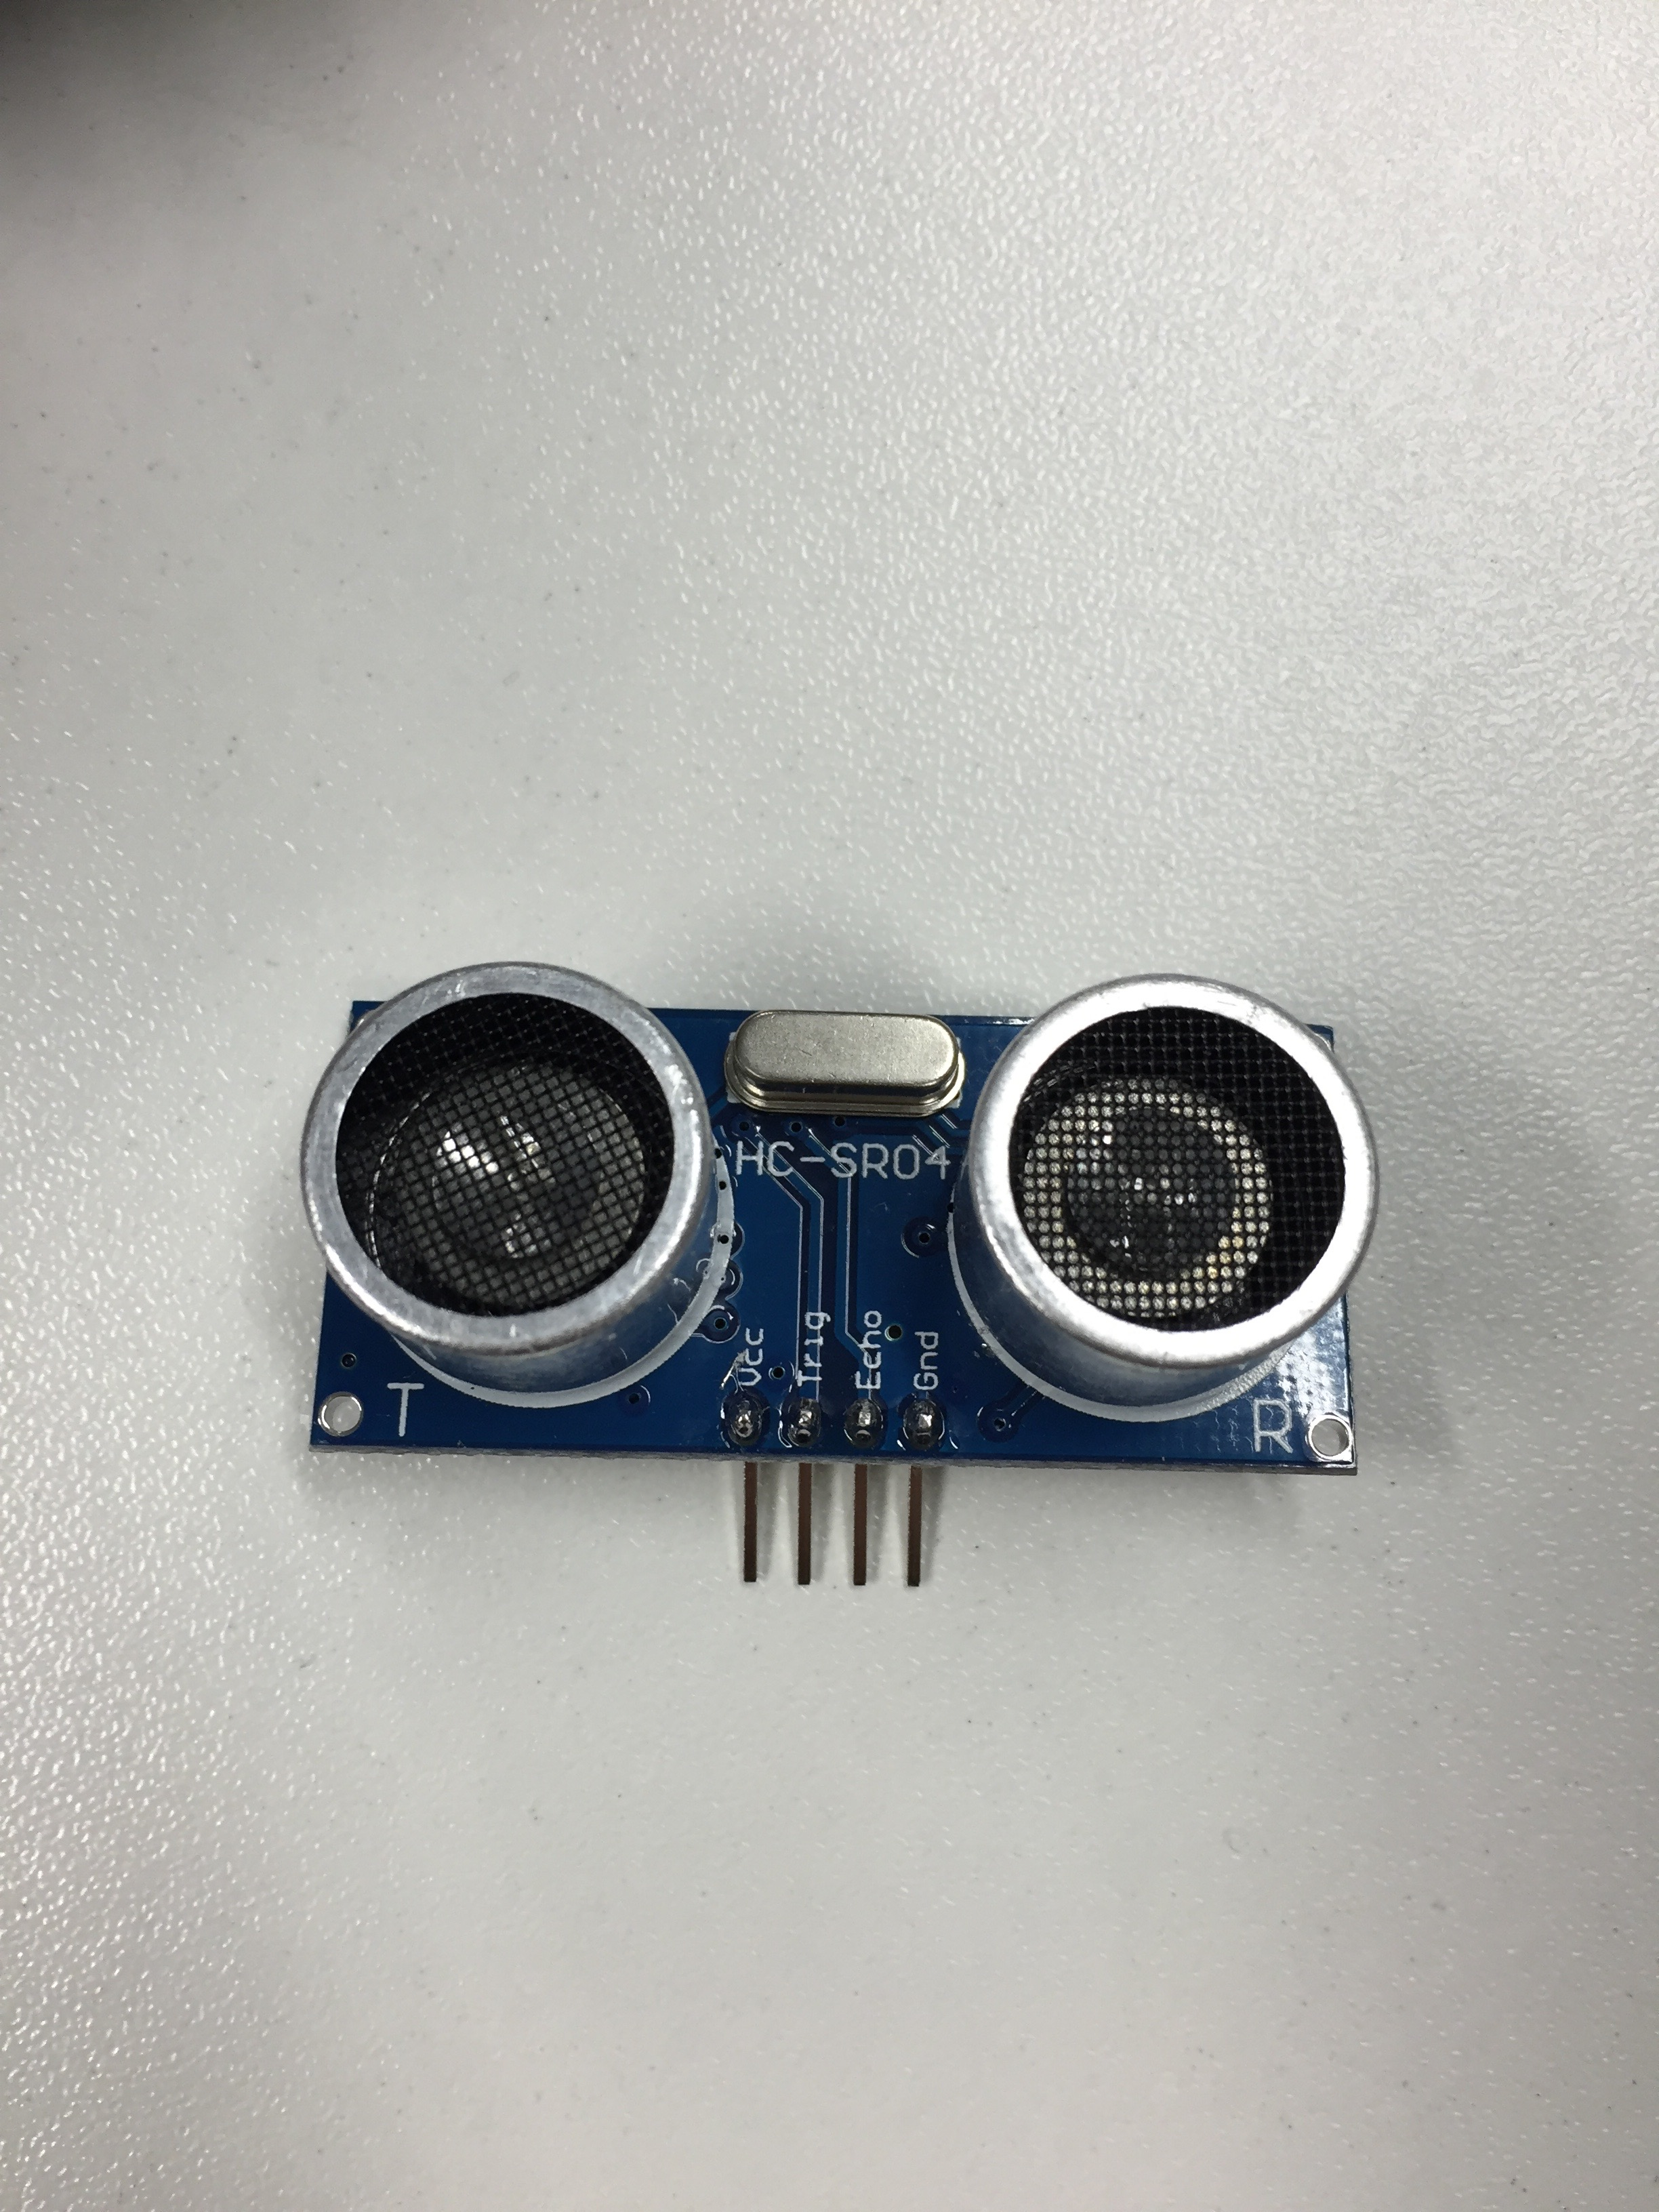
\includegraphics[trim={14cm 30cm 14cm 50cm}, clip, width=2.6in]{./media/Sonar.jpg}
\end{figure}
The robot uses a sonar to detect obstacles. 
The sonar consists of a transmitter that sends out ultrasonic waves and a receiver which detects the reflection of these waves.
\newpage
\begin{wrapfigure}{l}{7cm}
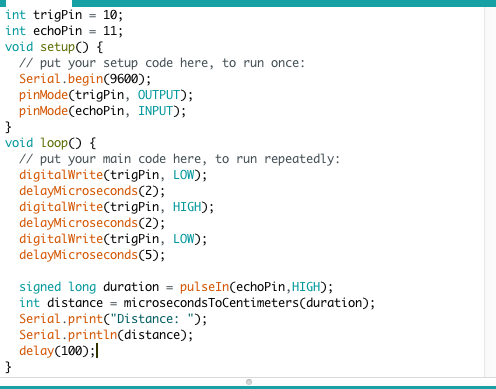
\includegraphics[trim={0cm 0cm 0cm 0cm}, clip, width=2.6in]{./media/sonarCode.jpg}
\end{wrapfigure}%
The setup part is to "set up" the communication between sonar and Arduino.
In the Loop part, we tell the sonar to send out a low signal followed by a high signal followed by a low signal.
Using the pulseIn function we get the time it took (in microseconds) for the receiver to detect the reflection if the high signal.\\ \\ \\ \\ \\ \\ \\

Finally, using the (self-defined) "microsecondsToCentimeters" function, we get the distanceat which the wave has been reflected.
\begin{figure}[!h]
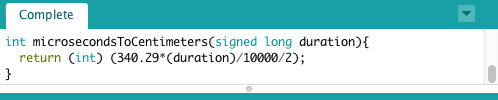
\includegraphics[trim={0cm 0cm 0cm 0cm}, clip, width=2.6in]{./media/sonarDistanceFunction.jpg}
\end{figure}

This next part of the code are the commands in case it does come near an obsticacle.
\begin{figure}[h!]
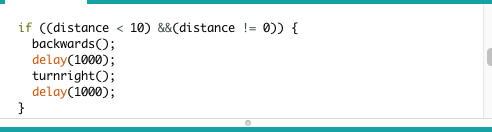
\includegraphics[trim={0cm 0cm 0cm 0cm}, clip, width=3in]{./media/obstacleAvoidance.jpg}
\end{figure}
It basically says: "when you get within 10cm of an object, go back a little and change direction".

\section{Light Follower}
\begin{figure}[h!]
\includegraphics[trim={0cm 0cm 0cm 0cm}, clip, width=2.6in, height=1.8in]{./media/ldr.png}
\end{figure}
To detect changes in Light intensity, I used two light dependent resistors (LDR's).
\newpage
\begin{wrapfigure}{l}{8cm}
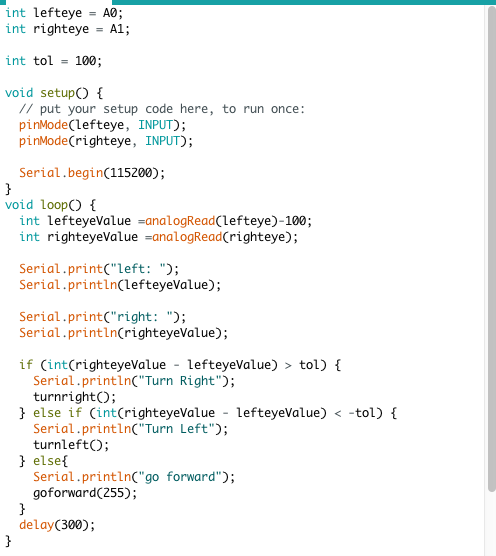
\includegraphics[trim={0cm 0cm 0cm 0cm}, clip, width=3in]{./media/lightFollower.jpg}
\end{wrapfigure}
In simple terms, this is how an LDR works:
Change in light intensity (arrow) change in resistance (arrow) change in voltage
The Arduino has a builtin analog-to-digital converter (ADC), with a 10 bit resolution.
This means at maximum light intensity, it will read the value 2pow(10)-1 (1023), and 0 when there is no light.
Decreasing the light intensity, increases the resistance and according to Ohm's law, also the voltage.
Therefore the side that reads reads a lower value will be the brighter one.
A tolerance of 50 seemed to work fine in a dark room. In a brighter room, you'll have decrease the tolerance (unless you have a ridiculously strong flash light).
Unfortunately, this made the robot more susceptible to unrelated sources of light. 

\end{document}
